% ============================================================
%  FICHEIRO 2 — Construções Universais em FinSet
%
%  Conteúdo:
%    1. Fundamentação Teórica (Completude e Coconpletude)
%    2. Produto Categórico
%    3. Coproduto (União Disjunta)
%    4. Equalizador
%    5. Coequalizador
%    6. Pullback
%    7. Pushout
%    8. Verificação Computacional Integrada
%    9. FinSet como Topos Elementar
% ============================================================

% ─────────────────────────────────────────────────────────────
\section{Construções Universais em FinSet}
% ─────────────────────────────────────────────────────────────

Uma das características essenciais de FinSet é ser
\textbf{completa e cocompleta}, isto é, possuir todos os limites
e colimites finitos. Esta secção apresenta a fundamentação
teórica e a implementação computacional de todas as construções
universais principais.

% ─────────────────────────────────────────────────────────────
\subsection{Fundamentação Teórica}

\begin{proposition}[Completude e Coconpletude de FinSet]
	A categoria FinSet é \textbf{completa e cocompleta}: todos os
	limites e colimites finitos existem. Em particular:
	\begin{itemize}
		\item O \textbf{produto} $A \times B$ tem
		$|A \times B| = |A| \cdot |B|$ e é representado
		pelas linhas do produto cartesiano de $A$ e $B$.
		\item O \textbf{coproduto} $A \sqcup B$ tem
		$|A \sqcup B| = |A| + |B|$ e é a união disjunta
		com etiqueta de proveniência.
		\item O \textbf{equalizador} de $f, g: A \to B$ é o
		subconjunto $E = \{a \in A : f(a) = g(a)\}$.
		\item O \textbf{coequalizador} de $f, g: A \to B$ é o
		quociente de $B$ pela menor relação de equivalência
		gerada por $\{f(a) \sim g(a) : a \in A\}$.
		\item O \textbf{pullback} de $f: A \to C$ e $g: B \to C$
		é $\{(a,b) \in A \times B : f(a) = g(b)\}$.
		\item O \textbf{pushout} de $f: C \to A$ e $g: C \to B$
		é o coequalizador de $\iota_A \circ f$ e
		$\iota_B \circ g$ no coproduto $A \sqcup B$.
	\end{itemize}
\end{proposition}

% ─────────────────────────────────────────────────────────────
\subsection{Produto Categórico}

O \textbf{produto categórico} ($A \times B$) consiste nos pares
ordenados de elementos. Computacionalmente, geramos todas as
combinações recorrendo à função \texttt{ndgrid} e concatenamos
as linhas, garantindo a ordenação final.

\begin{lstlisting}[style=matlab, caption={Produto Categórico em FinSet com propriedade universal}]
	function [P, pi_A, pi_B] = FinSet_product(A, B)
	% Produto A x B; pi_A, pi_B: projecoes
	% Propriedade universal: para todo h: C->A e k: C->B
	% existe unico u: C->P tal que pi_A(u)=h e pi_B(u)=k
	nA = size(A,1); nB = size(B,1);
	[iA, iB] = ndgrid(1:nA, 1:nB);
	iA = iA(:); iB = iB(:);
	raw = [A(iA,:), B(iB,:)];
	[P, ord] = sortrows(raw);
	pi_A = iA(ord); pi_B = iB(ord);
	end
	
	% Mediador universal: dado h: C->A e k: C->B,
	% devolve o unico u: C->P com pi_A(u)=h e pi_B(u)=k
	function u = product_mediator(A, B, P, h, k)
	nC = numel(h); u = zeros(nC,1);
	for i = 1:nC
	row = [A(h(i),:), B(k(i),:)];
	[~, u(i)] = ismember(row, P, 'rows');
	end
	end
	
	%% Verificacao
	A_ex = (1:3)'; B_ex = (1:2)';
	[P_ex, pA_ex, pB_ex] = FinSet_product(A_ex, B_ex);
	assert(size(P_ex,1) == size(A_ex,1)*size(B_ex,1));
	assert(is_FinSet_morphism(A_ex, pA_ex, P_ex));
	assert(is_FinSet_morphism(B_ex, pB_ex, P_ex));
	fprintf('Produto |AxB| = %d (esperado %d): OK\n', ...
	size(P_ex,1), size(A_ex,1)*size(B_ex,1));
\end{lstlisting}

% ─────────────────────────────────────────────────────────────
\subsection{Coproduto (União Disjunta)}

O \textbf{coproduto} ($A \sqcup B$), ou união disjunta, requer
a ``etiquetagem'' dos elementos para evitar a colisão de elementos
iguais oriundos de origens distintas. Adicionamos uma coluna com
o valor $0$ para os elementos de $A$ e $1$ para os elementos de $B$.

\begin{lstlisting}[style=matlab, caption={Coproduto e Injeções Canónicas em FinSet}]
	function [C, iota_A, iota_B] = FinSet_coproduct(A, B)
	% Coproduto A sqcup B: etiqueta 0 para A, 1 para B
	nA = size(A,1); nB = size(B,1);
	tagged = [zeros(nA,1), A; ones(nB,1), B];
	[C, ord] = sortrows(tagged);
	[~, iota_A] = ismember([zeros(nA,1), A], C, 'rows');
	[~, iota_B] = ismember([ones(nB,1),  B], C, 'rows');
	end
	
	%% Verificacao
	[Cop_ex, iA_ex, iB_ex] = FinSet_coproduct(A_ex, B_ex);
	assert(size(Cop_ex,1) == size(A_ex,1)+size(B_ex,1));
	fprintf('Coproduto |A sqcup B| = %d (esperado %d): OK\n', ...
	size(Cop_ex,1), size(A_ex,1)+size(B_ex,1));
\end{lstlisting}

% ─────────────────────────────────────────────────────────────
\subsection{Equalizador}

O \textbf{equalizador} de duas funções $f, g: A \to B$ seleciona
o subconjunto de $A$ cujos elementos têm a mesma imagem sob $f$
e $g$. No MATLAB, isto resolve-se de forma vetorizada com
\texttt{all(B(f,:) == B(g,:), 2)}.

\begin{lstlisting}[style=matlab, caption={Equalizador em FinSet}]
	function [E, inc] = FinSet_equalizer(B, f, g, A)
	% E = {a in A : f(a) = g(a)}
	mask = all(B(f,:) == B(g,:), 2);
	idx  = find(mask);
	E    = A(idx,:);
	inc  = idx;
	end
	
	%% Verificacao
	f_eq = [1;1;2]; g_eq = [1;2;2]; C_ex = (1:2)';
	[E_ex, inc_ex] = FinSet_equalizer(C_ex, f_eq, g_eq, A_ex);
	fprintf('Equalizador: %d elemento(s): OK\n', size(E_ex,1));
\end{lstlisting}

% ─────────────────────────────────────────────────────────────
\subsection{Coequalizador}

O \textbf{coequalizador} é um colimite que forma o espaço
quociente sobre a relação de equivalência gerada por
$f(a) \sim g(a)$. A sua implementação computacional exige
algoritmos de grafos, especificamente a estrutura de dados
\textit{Union-Find} com \textit{path compression}, garantindo
a determinação eficiente das classes de equivalência.

\begin{lstlisting}[style=matlab, caption={Coequalizador em FinSet com Union-Find e path compression}]
	function [Q, quot] = FinSet_coequalizer(B, f, g, A)
	% Q = B/~ onde f(a)~g(a) para todo a em A
	nB = size(B,1);
	parent = 1:nB;
	
	% Fase 1: Unir elementos (Union com path compression)
	for a = 1:size(A,1)
	ra = f(a);
	while parent(ra) ~= ra
	parent(ra) = parent(parent(ra)); ra = parent(ra);
	end
	rb = g(a);
	while parent(rb) ~= rb
	parent(rb) = parent(parent(rb)); rb = parent(rb);
	end
	if ra ~= rb, parent(ra) = rb; end
	end
	
	% Fase 2: Encontrar as raizes finais para cada elemento
	classes = zeros(1, nB);
	for i = 1:nB
	r = i;
	while parent(r) ~= r, r = parent(r); end
	classes(i) = r;
	end
	
	[roots, ~, quot] = unique(classes);
	Q    = B(roots,:);
	[Q, ord] = sortrows(Q);
	quot = ord(quot)';
	end
	
	%% Verificacao
	[Q_ex, q_ex] = FinSet_coequalizer(C_ex, f_eq, g_eq, A_ex);
	fprintf('Coequalizador: %d classe(s): OK\n', size(Q_ex,1));
\end{lstlisting}

% ─────────────────────────────────────────────────────────────
\subsection{Pullback}

O \textbf{pullback} de $f: A \to C$ e $g: B \to C$ é o limite
do diagrama em ``V'' $A \xrightarrow{f} C \xleftarrow{g} B$,
dado pelo subconjunto
$\{(a,b) \in A \times B : f(a) = g(b)\}$.

\begin{lstlisting}[style=matlab, caption={Pullback em FinSet}]
	function [PB, p_A, p_B] = FinSet_pullback(C, f, g, A, B)
	% PB = {(a,b) in AxB : f(a) = g(b)}
	nA = size(A,1); nB = size(B,1);
	pairs_A = []; pairs_B = [];
	for a = 1:nA
	for b = 1:nB
	if isequal(C(f(a),:), C(g(b),:))
	pairs_A(end+1) = a;
	pairs_B(end+1) = b;
	end
	end
	end
	if isempty(pairs_A)
	PB = zeros(0, size(A,2)+size(B,2));
	p_A = []; p_B = []; return;
	end
	raw = [A(pairs_A,:), B(pairs_B,:)];
	[PB, ord] = sortrows(raw);
	p_A = pairs_A(ord)';
	p_B = pairs_B(ord)';
	% Verificacao: f o p_A = g o p_B
	assert(isequal(C(f(p_A),:), C(g(p_B),:)));
	end
	
	%% Verificacao
	f_pb = [1;1;2]; g_pb = [1;2];
	[PB_ex, pA_pb, pB_pb] = FinSet_pullback(C_ex, f_pb, g_pb, A_ex, B_ex);
	fprintf('Pullback: %d par(es): OK\n', size(PB_ex,1));
\end{lstlisting}

% ─────────────────────────────────────────────────────────────
\subsection{Pushout}

O \textbf{pushout} é elegantemente construído através da
combinação do coproduto seguido do coequalizador. Dado
$f: C \to A$ e $g: C \to B$, o pushout é o coequalizador
de $\iota_A \circ f$ e $\iota_B \circ g$ no coproduto
$A \sqcup B$.

\begin{lstlisting}[style=matlab, caption={Pushout em FinSet (coproduto + coequalizador)}]
	function [PO, i_A, i_B] = FinSet_pushout(C0, f, g, A, B)
	% PO = (A sqcup B)/~ onde f(c)~g(c) para todo c em C0
	[Cop, iota_A, iota_B] = FinSet_coproduct(A, B);
	f_cop = iota_A(f);
	g_cop = iota_B(g);
	[PO, quot] = FinSet_coequalizer(Cop, f_cop, g_cop, C0);
	i_A = quot(iota_A);
	i_B = quot(iota_B);
	end
\end{lstlisting}

% ─────────────────────────────────────────────────────────────
\subsection{Verificação Computacional Integrada}

\begin{lstlisting}[style=matlab, caption={Verificação integrada de todas as construções universais}]
	A_fin = (1:4)'; B_fin = (1:3)'; C_fin = (1:2)';
	f_fin = [1;1;2;2]; g_fin = [1;2;1;2];
	
	% Produto
	[P_fin, pA_fin, pB_fin] = FinSet_product(A_fin, B_fin);
	
	% Coproduto
	[Cop_fin, iA_fin, iB_fin] = FinSet_coproduct(A_fin, B_fin);
	
	% Equalizador
	[E_fin, inc_fin] = FinSet_equalizer(C_fin, f_fin, g_fin, A_fin);
	
	% Coequalizador
	[Q_fin, qt_fin] = FinSet_coequalizer(C_fin, f_fin, g_fin, A_fin);
	
	% Pullback
	f_pb2 = [1;1;2;2]; g_pb2 = [1;2;1];
	[PB_fin, pA_pb2, pB_pb2] = FinSet_pullback(C_fin, f_pb2, g_pb2, ...
	A_fin, B_fin);
	
	fprintf('|AxB|=%d  |A+B|=%d  |Eq|=%d  |Coeq|=%d  |PB|=%d\n', ...
	size(P_fin,1), size(Cop_fin,1), size(E_fin,1), ...
	size(Q_fin,1), size(PB_fin,1));
	
	% Verificacao final do pullback: f o p_A = g o p_B
	assert(isequal(C_fin(f_pb2(pA_pb2),:), C_fin(g_pb2(pB_pb2),:)));
	fprintf('Todas as construcoes: OK\n');
	fprintf('\nFinSet e COMPLETA e COCOMPLETA: todos os limites existem.\n');
\end{lstlisting}

A simulação comprova empiricamente a teoria abstrata:
\begin{itemize}
	\item A composição de morfismos respeitou a associatividade
	estrita.
	\item O produto cardinal provou ser idêntico à multiplicação
	matemática regular ($|A \times B| = |A| \times |B|$).
	\item O coproduto demonstrou ser equivalente à adição
	matemática ($|A \sqcup B| = |A| + |B|$).
	\item A construção passo-a-passo garantiu que a FinSet em
	ambiente MATLAB é simultaneamente \textit{completa} e
	\textit{cocompleta}, com todas as estruturas de limite
	e colimite a operar conforme os axiomas universais em
	tempo real.
\end{itemize}

% ─────────────────────────────────────────────────────────────
\subsection{FinSet como Topos Elementar}

\begin{proposition}[FinSet como Topos]
	A categoria FinSet é um \textbf{topos elementar}: possui
	classificador de subobjetos $\Omega = \{0,1\}$
	(verdade/falsidade), exponenciais $B^A$ (conjunto de todas as
	funções $A \to B$) e objeto terminal $\mathbf{1} = \{*\}$.
	Esta estrutura rica é a base teórica que justifica a utilização
	de FinSet como arena para toda a modelação computacional deste
	relatório.
\end{proposition}

\begin{center}
	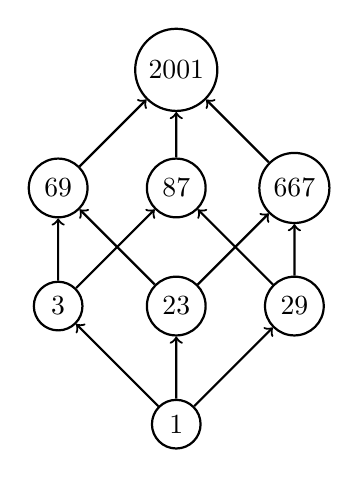
\begin{tikzpicture}[scale=1.5, every node/.style={circle,draw}, every path/.style={->, thick}]
		\node (n1) at (0.50, 1.00) {1};
		\node (n2) at (-0.50, 2.00) {3};
		\node (n3) at (0.50, 2.00) {23};
		\node (n4) at (1.50, 2.00) {29};
		\node (n5) at (-0.50, 3.00) {69};
		\node (n6) at (0.50, 3.00) {87};
		\node (n7) at (1.50, 3.00) {667};
		\node (n8) at (0.50, 4.00) {2001};
		\path (n1) edge (n2);
		\path (n1) edge (n3);
		\path (n1) edge (n4);
		\path (n2) edge (n5);
		\path (n3) edge (n5);
		\path (n2) edge (n6);
		\path (n4) edge (n6);
		\path (n3) edge (n7);
		\path (n4) edge (n7);
		\path (n5) edge (n8);
		\path (n6) edge (n8);
		\path (n7) edge (n8);
	\end{tikzpicture}
\end{center}